\documentclass[a4paper,12pt, oneside]{book}

% \usepackage{fullpage}
\usepackage[italian]{babel}
\usepackage[utf8]{inputenc}
\usepackage{amssymb}
\usepackage{amsthm}
\usepackage{graphics}
\usepackage{amsfonts}
\usepackage{listings}
\usepackage{amsmath}
\usepackage{amstext}
\usepackage{engrec}
\usepackage{rotating}
\usepackage{verbatim}
\usepackage[safe,extra]{tipa}
\usepackage{multirow}
\usepackage{hyperref}
\usepackage{microtype}
\usepackage{fontspec}
\usepackage{enumerate}
\usepackage{physics}
\usepackage{braket}
\usepackage{marginnote}
\usepackage{pgfplots}
\usepackage{cancel}
\usepackage{polynom}
\usepackage{booktabs}
\usepackage{enumitem}
\usepackage{framed}
\usepackage{pdfpages}
\usepackage{pgfplots}
\usepackage{algorithm}
% \usepackage{algpseudocode}
\usepackage[cache=false]{minted}
\usepackage{mathtools}
\usepackage[noend]{algpseudocode}
\newcommand*{\bfrac}[2]{\genfrac{}{}{0pt}{}{#1}{#2}}

\usepackage{tikz}\usetikzlibrary{er}\tikzset{multi  attribute /.style={attribute
    ,double  distance =1.5pt}}\tikzset{derived  attribute /.style={attribute
    ,dashed}}\tikzset{total /.style={double  distance =1.5pt}}\tikzset{every
  entity /.style={draw=orange , fill=orange!20}}\tikzset{every  attribute
  /.style={draw=MediumPurple1, fill=MediumPurple1!20}}\tikzset{every
  relationship /.style={draw=Chartreuse2,
    fill=Chartreuse2!20}}\newcommand{\key}[1]{\underline{#1}}
\usetikzlibrary{arrows.meta}
\usetikzlibrary{decorations.markings}
\usetikzlibrary{arrows,shapes,backgrounds,petri}
\tikzset{
  place/.style={
    circle,
    thick,
    draw=black,
    minimum size=6mm,
  },
  transition/.style={
    rectangle,
    thick,
    fill=black,
    minimum width=8mm,
    inner ysep=2pt
  },
  transitionv/.style={
    rectangle,
    thick,
    fill=black,
    minimum height=8mm,
    inner xsep=2pt
  }
} 
\usetikzlibrary{automata,positioning,chains,fit,shapes}
\usepackage{fancyhdr}
\pagestyle{fancy}
\fancyhead[LE,RO]{\slshape \rightmark}
\fancyhead[LO,RE]{\slshape \leftmark}
\fancyfoot[C]{\thepage}
\usepackage[usenames,dvipsnames]{pstricks}
\usepackage{epsfig}
\usepackage{pst-grad} % For gradients
\usepackage{pst-plot} % For axes
\usepackage[space]{grffile} % For spaces in paths
\usepackage{etoolbox} % For spaces in paths
\makeatletter % For spaces in paths
\patchcmd\Gread@eps{\@inputcheck#1 }{\@inputcheck"#1"\relax}{}{}
\makeatother
\usepackage{lipsum}
\DeclareSymbolFont{symbolsC}{U}{txsyc}{m}{n}
\DeclareMathSymbol{\strictif}{\mathrel}{symbolsC}{74}
\title{Data and Computational Biology}
\author{UniShare\\\\Davide Cozzi\\\href{https://t.me/dlcgold}{@dlcgold}}
\date{}

\pgfplotsset{compat=1.13}
\begin{document}
\maketitle

\definecolor{shadecolor}{gray}{0.80}
\setlist{leftmargin = 2cm}
\newtheorem{teorema}{Teorema}
\newtheorem{definizione}{Definizione}
\newtheorem{esempio}{Esempio}
\newtheorem{corollario}{Corollario}
\newtheorem{lemma}{Lemma}
\newtheorem{osservazione}{Osservazione}
\newtheorem{nota}{Nota}
\newtheorem{esercizio}{Esercizio}
\algdef{SE}[DOWHILE]{Do}{doWhile}{\algorithmicdo}[1]{\algorithmicwhile\ #1}
\tableofcontents
\renewcommand{\chaptermark}[1]{%
  \markboth{\chaptername
    \ \thechapter.\ #1}{}}
\renewcommand{\sectionmark}[1]{\markright{\thesection.\ #1}}
\newcommand{\floor}[1]{\lfloor #1 \rfloor}
\newcommand{\MYhref}[3][blue]{\href{#2}{\color{#1}{#3}}}%
\chapter{Introduzione}
\textbf{Questi appunti sono presi a lezione. Per quanto sia stata fatta
  una revisione è altamente probabile (praticamente certo) che possano
  contenere errori, sia di stampa che di vero e proprio contenuto. Per
  eventuali proposte di correzione effettuare una pull request. Link: }
\url{https://github.com/dlcgold/Appunti}.\\
\chapter{Introduzione alla Biologia Computazionale}
\begin{shaded}
  \textbf{Materiale tratto dalla tesi}.\\
  \section{Accenni di biologia molecolare}
  \subsection{DNA ed RNA}
  Prima di iniziare la trattazione più squisitamente computazionale è bene dare
  un'introduzione, dal punto di vista biologico, di quanto trattato.\\
  Il \textbf{DNA}, sigla corrispondente ad \textbf{acido desossiribonucleico}, è
  un acido nucleico contenente le informazioni necessarie al corretto sviluppo di
  un essere vivente. Dal punto di vista chimico questa particolare macromolecola
  si presenta nella tipica \textbf{struttura a doppia elica}, formata da due
  lunghe catene di nucleotidi, dette \textbf{strand}. Nel dettaglio i singoli
  nucleotidi sono formati da un \textbf{gruppo fosfato}, dal
  \textbf{desossiribosio}, uno \textbf{zucchero pentoso,} e da una \textbf{base
  azotata}. Si hanno, inoltre, 4 tipi diversi di basi azotate:
  \begin{enumerate}
    \item \textbf{Adenina}, indicata con la lettera $A$
    \item \textbf{Citosina}, indicata con la lettera $C$
    \item \textbf{Guanina}, indicata con la lettera $G$
    \item \textbf{Timina}, indicata con la lettera $T$
  \end{enumerate}
  Si hanno quindi due \textbf{strand}, uno detto \textbf{forward
  strand} (indicato solitamente col simbolo ``+'') e uno detto \textbf{backward
  strand} (indicato solitamente col simbolo ``$-$'') che sono direzionati nel
  verso  
  opposto (in termini tecnici si ha che il forward strand va da 5' UTR a 3' UTR,
  mentre il backward strand da 3' UTR a 5' UTR) e sono \textit{appaiati} mediante
  coppie ben precise di basi azotate.
  Infatti, secondo il \textbf{modello di Watson-Crick}, si
  ha che:  
  \begin{itemize}
    \item l'\textbf{Adenina} si appaia con la \textbf{Timina} e viceversa
    \item la \textbf{Citosina} si appaia con la \textbf{Guanina} e viceversa
  \end{itemize}
  Questo accoppiamento permette di poter studiare i due \textbf{strand} come uno
  ``complementare'' all'altro. Infatti, conoscendo la sequenza di basi azotate
  di 
  uno \textbf{strand}, è possibile ricavare la sequenza dell'altro mediante la
  tecnica del \textbf{Reverse}\&\textbf{Complement} dove, preso uno strand, si
  converte ogni sua base secondo il seguente schema:
  \begin{itemize}
    \item le $A$ diventano $T$
    \item le $T$ diventano $A$
    \item le $C$ diventano $G$
    \item le $G$ diventano $C$
  \end{itemize}
  \begin{esempio}
    Vediamo, per completezza, un esempio di
    \textbf{Reverse}\textnormal{\&}\textbf{Complement}.\\ 
    Prendiamo una sequenza genomica $S="\mbox{TAGGCCATATGAC}\,"$ e definiamo la
    funzione 
    $RC(x)$ come la funzione che, presa in ingresso una stringa $x$ costruita
    sull'alfabeto $\Sigma=\{A,C,G,T\}$ (quindi una sequenza genomica),
    restituisce 
    la \textbf{Reverse}\textnormal{\&}\textbf{Complement} della stessa. Si ha
    quindi che: 
    \[RC(S)="\mbox{ATCCGGTATACTG}\,"\]
  \end{esempio}
  Per riferirci al \textbf{DNA}, contenuto in una data cellula di un essere
  vivente, usiamo il termine \textbf{genoma}, che a sua volta viene organizzato
  in 
  diversi \textbf{cromosomi}. Si definisce \textbf{gene} una particolare regione
  di un \textbf{cromosoma} in grado di codificare una proteina. \\
  Ai fini della trattazione del progetto, è necessario introdurre anche
  l'\textbf{RNA}, sigla corrispondente ad \textbf{acido ribonucleico} (avendo il
  \textbf{ribosio} come zucchero pentoso), ovvero una
  molecola, simile al \textbf{DNA}, dotata di una singola 
  catena nucleotidica, sempre con 4 tipi di basi azotate (anche se si ha
  l'\textbf{Uracile}, che si indica con la lettera $U$, al posto della
  \textbf{Timina}). Tra i compiti dell'\textbf{RNA} si ha quello della codifica
  e 
  decodifica dei \textbf{geni}.
  \subsection{Esoni, Introni e Splicing alternativo}
  Per ottenere una \textbf{proteina} da un \textbf{gene} si hanno 3 passaggi:
  \begin{enumerate}
    \item La \textbf{trascrizione}, fase dove la sequenza del gene è copiata
    nel \textbf{pre-messenger RNA (pre-mRNA)}. Nel dettaglio viene selezionato
    uno 
    dei due strand del gene e un enzima, chiamato \textbf{RNA Polimerasi},
    procede 
    alla trascrizione della sequenza selezionata creando il
    \textbf{pre-mRNA}. In
    questa fase la \textit{Timina} viene sostituita dall'Uracile. È bene
    introdurre subito che in questo progetto non si terrà mai conto, a fini di
    semplificazione, del passaggio tra Timina e Uracile in quanto verrà usata
    sempre la \textit{Timina}.
    \item Lo \textbf{splicing}, fase dove vengono rimosse le parti non
    codificanti 
    dalla molecola di \textbf{pre-mRNA}, formando il \textbf{messenger RNA
      (mRNA)},
    detto anche \textbf{trascritto}. Per poter trattare al meglio questa fase
    bisogna parlare in primis di \textbf{esoni} e \textbf{introni}. In prima
    analisi si potrebbe dire, peccando di precisione, che gli
    \textbf{esoni} sono le sezioni codificanti di un gene mentre gli
    \textbf{introni} sono le porzioni non codificanti. Solo gli esoni formano il
    trascritto. Si ha, inoltre, che le prime due basi di un introne sono dette
    $5'$, nell'uomo solitamente si ha la coppia $GT$, mentre le ultime due,
    solitamente $AG$ nell'uomo, sono
    dette $3'$ e sono meglio identificate come \textbf{siti di taglio (splice
      sites)}. 
    Quindi un esone, in realtà, non coincide esattamente con una regione
    codificante, detta \textbf{CDS}, a causa di queste particolari coppie di
    basi. Si notifica però che, come spesso accade, i termini vengono usati in
    sovrapposizione. 
    \item La \textbf{traduzione}, fase dove viene effettivamente codificata la
    proteina a partire da una sezione dell'\textbf{m-RNA}. 
    Bisogna quindi nominare particolari sequenze nucleotidiche di cardinalità 3:
    i 
    \textbf{codoni}. Tali triplette sono tradotte in amminoacidi che,
    concatenati, 
    formano le proteine. Esistono particolari codoni che sono utili al fine
    di riconoscere l'inizio e la fine della \textit{sintesi proteica}. In
    particolare si ha un codone d'inizio, detto \textbf{start codon}, che
    solitamente corrisponde alla tripletta \textit{AUG}, mentre, per il codone
    di 
    fine, detto \textbf{stop codon}, solitamente si ha una tripletta tra
    \textit{UAA}, \textit{UAG} e  \textit{UGA}.
  \end{enumerate}
  In realtà, un gene è in grado di sintetizzare più di una proteina
  mediante il cosiddetto \textbf{splicing alternativo}, che consiste in diverse
  varianti dell'evento di splicing al fine di ottenere diversi trascritti. Si
  descrivono le principali modalità di splicing alternativo:
  \begin{itemize}
    \item L'\textbf{exon skipping}, ovvero \textit{salto dell'esone}, dove un
    esone 
    (o anche più esoni) può essere escluso dal trascritto primario oppure dove
    un 
    nuovo esone (o più nuovi esoni) può essere incluso nello stesso. 
    \item L'\textbf{alternative acceptor site}, ovvero \textit{sito di taglio
      alternativo $3'$}, dove una parte del secondo esone può essere considerata
    non codificante o, alternativamente, una porzione dell'introne adiacente può
    essere considerata codificante.
    \item L'\textbf{alternative donor site}, ovvero \textit{sito di taglio
      alternativo $5'$}, dove una parte del primo esone viene considerata non
    codificante o, alternativamente, una porzione di introne adiacente può
    essere considerata codificante.
    \item I \textbf{mutually exclusive exons}, ovvero \textit{esoni mutuamente
      esclusivi}, dove solo uno di due esoni viene conservato nel trascritto.
    \item L'\textbf{intron retention}, ovvero \textit{introne trattenuto}, dove
    un 
    certo introne viene incluso nel trascritto primario.
  \end{itemize}
  Le varie modalità di splicing alternativo non si escludono a vicenda, rendendo
  lo studio di tale fenomeno assai complesso.
\end{shaded}
La \textbf{biologia} nasce come una disciplina altamente \textbf{descrittiva}
mentre altre discipline, come, ad esempio, informatica, matematica o fisica,
sono discipline \textbf{generaliste}. In biologia infatti si parte dai dati e
dagli esperimenti per descrivere un fenomeno ed inferire la teoria su di
esso. Questo è un discorso più di \textbf{filosofia della scienza}.\\
I biologi propongono \textbf{modelli}, come ad esempio i \textit{pathway}, che
sono il diretto risultato di osservazioni sperimentali e interpretazione dei
risultati.
\begin{definizione}
  Un \textbf{pathway (\emph{percorso}) biologico} è una serie di interazioni
  tra molecole in una cellula che porta a un determinato prodotto o un
  cambiamento in una cellula. Tale \emph{percorso} può innescare
  l'assemblaggio di nuove molecole, come un grasso o una proteina. I
  \emph{percorsi} possono anche attivare e disattivare i geni o stimolare una
  cellula a muoversi. I pathway più comuni sono coinvolte nel metabolismo, nella
  regolazione dell'espressione genica e nella trasmissione dei segnali e
  svolgono un ruolo chiave negli studi avanzati di genomica.\\
  Tra le principali categorie si hanno:
  \begin{itemize}
    \item Metabolic pathway
    \item Genetic pathway
    \item Signal transduction pathway
  \end{itemize}
\end{definizione}
Un altro aspetto chiave negli ultimi 25 anni è stato quello della
mole di dati prodotti, tramite, ad esempio, \textbf{Next Generation Sequencing
  (\textit{NGS})}, con la produzione di \textit{DNAseq} e \textit{RNAseq} (che
rispetto alle \textit{DNAseq} sono più semplici da sequenziare e studiare e
servono a vedere cosa sintetizza effettivamente una cellula), o
alla cosiddetta \textbf{single-cell analysis}, una tecnica più recente,
sviluppata negli ultimi 5 anni. I costi di sequenziamento variano a seconda
del numero di basi da sequenziare ed è in calo negli anni.
Tutte queste tecnologie 
\textit{high-throughput} usate in biologia computazionale e in bioinformatica
richiedono una forte conoscenza algoritmica, matematica e statistica per la
gestione di questa enorme quantità di dati (essendo anche nell'ambito
\textbf{big data}) in ambito biomedico. Saper modellare fenomeni biologici è
essenziale anche per poter capire come eventualmente funzionano tecniche di
machine learning dedicate, come le reti neurali. Ovviamente le conoscenze, i
tempi (ma anche gli spazi), gli strumenti da usare e sviluppare etc$\ldots$ variano al
variare del tipo di studio. Ad ogni problema è associato un miglior strumento di
modellistica.\\ 
Un altro aspetto non trascurabile è la scala di misura di ciò che viene
studiato, ad esempio:
\begin{itemize}
  \item \textit{organismi}, ad esempio per gli organismi multicellulari si passa
  da $10\mu m$ a $50/85m$ 
  \item \textit{tessuti}, ad esempio per i tessuti umani siamo in un range
  maggiore di $10^4 \mu m^3$
  \item \textit{cellule}, ad esempio per quelle umane si va da $30\mu m^3$ a
  $10^6 \mu m^3$ con:
  \begin{itemize}
    \item membrane
    \item nuclei
    \item ribosomi
    \item mitocondri e cloroplasti
    \item altri organelli e strutture intracellulari
    \item proteine
    \item materiale genomico (DNA e RNA e affini strutture: ad esempio istoni) 
    \item $\ldots$
  \end{itemize}
\end{itemize}
Parlando di tipi di organismi distinguiamo in primis:
\begin{itemize}
  \item \textbf{eucarioti}. In questo caso si hanno cellule più complesse, con
  numerosi organelli e soprattutto il \textbf{nucleo}, dove sono contenute le
  informazioni. Si hanno i \textbf{mitocondri}, che si occupano di generare
  \textit{energia} tramite \textit{glicolisi} e sono studiati in ambito
  filogenetico, in quanto provengono 
  unicamente dalla madre, permettendo la \textit{filogenesi materna}
  \item \textbf{procarioti}, come i \textit{batteri}. In questo caso si hanno
  cellule piccole e semplici. Non hanno un nucleo ma solo una regione, detta
  \textbf{nucleoide}, dove sono contenute le informazioni
\end{itemize}
Si hanno cellule nell'uomo, come quelle del sangue, dove non si ha un nucleo e
non si ha riproduzione. D'altro canto si hanno anche cellule, come quelle
dell'occhio, che non cambiano mai nel corso della vita.\\
In aggiunta si hanno anche i cosiddetti \textbf{archaea}.\\
\begin{shaded}
  \textbf{Tratto da Wikipedia}.\\
  \textit{Gli archèi o archèobatteri, nome scientifico Archaea (dal termine del
  greco antico che significa antico) o Archaeobacteria che significa "batteri
  antichi", sono 
  una suddivisione sistematica della vita cellulare. Possono considerarsi regno
  o dominio a seconda degli schemi classificativi, ma mostrano strutture
  biochimiche tali da considerarsi un ramo basilare, presto distaccatosi dalle
  altre forme dei viventi. Nonostante il nome attribuito a questo taxon, gli
  archaea non sono i procarioti più antichi mai apparsi sulla Terra, ma sono
  stati preceduti dagli eubatteri.
  Essendo costituiti da singole cellule mancanti di nucleo, per forma e
  dimensioni 
  molto simili ai batteri, sono stati in passato classificati come procarioti o
  monere assieme ad essi. Originariamente furono ritrovati negli ambienti più
  estremi, ma successivamente sono stati trovati in tutti gli habitat, compreso
  l'intestino umano, nel caso del Methanobrevibacter smithii.\\
  Nonostante non sia del tutto sicura la filogenesi del gruppo, gli archei sono
  quindi (insieme agli eucarioti e agli eubatteri) uno dei tre fondamentali
  gruppi degli esseri viventi nella classificazione di Woese. Tesi recenti
  propongono di considerare Archea ed Eukaryota un unico regno, contrapposto ai
  Bacteria, in quanto all'origine degli eucarioti vi sarebbe l'endosimbiosi
  mitocondriale.}  
\end{shaded}
\textit{Per ulteriori informazioni sui tipi di organismi guardare online}.\\
Parlando di DNA si ha che ogni cellula umana contiene circa 2 metri di DNA e un
organismo umano contiene moltissime cellule rendendo lo studio del DNA davvero
complesso (anche dal punto di vista computazionale si hanno file di genomi
davvero molto pesanti, di centinaia di \textit{MB}). Si hanno migliaia di
trilioni di cellule nell'uomo.\\
Uno dei problemi è ``allungare'' il DNA che normalmente è incredibilmente
avvolto su se stesso (e solo in fase di divisione cellulare si riconosce la
forma a ``X'' dei cromosomi, altrimenti è ancora più avvolto su se stesso). \\
Dal DNA, nel nucleo, si ottiene l'RNA che esce, verso il citoplasma, dove, nei
ribosomi, viene usato per sintetizzare le proteine.\\
Si hanno alcune specie interessanti dal punto di vista genomico e modellistico:
\begin{itemize}
  \item \textbf{Saccharomyces cerevisiae}, ovvero il lievito da birra, con un
  piccolo genoma, \textit{12 Mb}
  \item \textbf{Caenorhabditis elegans}, un ``verme'' di cui si è studiato
  l'intero sviluppo. Gli esemplari femmina hanno poco meno di mille cellule,
  959, mentre i maschi poco di più, 1033. Si ha un genoma di \textit{97 Mb}
  \item \textbf{Drosophila melanogaster} un altro modello molto usato, con un
  genoma di \textit{180 Mb}
  \item \textbf{Homo sapiens}, con un genoma di \textit{3200 Mb}
  \item \textbf{Mus musculus}, ovvero il topo, che ha un genoma molto simile a
  quello umano e quindi è molto usato negli studi in laboratorio. Si ha un
  genoma di \textit{3300 Mb} 
  \item \textbf{Arabidopsis thaliana}, ovvero la Veccia, che viene usata come
  modello base per studiare le piante. Si ha un genoma di \textit{125 Mb} 
  \item \textbf{Fritillaria assyriaca}, ovvero la Fritillaria, che ha il più
  lungo genoma conosciuto, di \textit{120000 Mb}. Le piante normalmente hanno un
  genoma più lungo a causa dell'evoluzione, in quanto conservano molte
  informazioni che potrebbero essergli utili in futuro, anche in un futuro molto
  lontano, dovendo sopravvivere anche al fatto che non possono muoversi
\end{itemize}
Ad essere interessanti non sono solo le dimensioni di ciò che viene studiato ma
anche i vari \textbf{tempi}. Vediamo una piccola tabella d'esempio:
\begin{table}[H]
  \small
  \centering
  \begin{tabular}{c|c|c}
    \textbf{Proprietà} & \textbf{E. coli} & \textbf{Uomo}\\
    \hline
    \hline
    diffusione di proteine in una cellula & $0.1 s$ & $\sim 100 s$\\
    \hline
    trascrizione di un gene & $\sim 1m$ ($80\frac{bp}{s}$) & $\sim 100 s$\\
    \hline
    generazione di una cellula & da $30 m$ a ore & da $20h$ a statico\\
    \hline
    transizione di stato proteico & da $1\mu s$ a $100\mu s$
                                          & da $1\mu s$ a $100\mu s$\\
    \hline
    rate di mutazione & $\sim \frac{10^{-9}}{\frac{bp}{generazione}}$
                                      & $\sim \frac{10^{-8}}{\frac{bp}{anno}}$\\
  \end{tabular}
\end{table}
Qualche nota:
\begin{itemize}
  \item i tempi di trascrizione di un gene umano includono i tempi di
  preprocessamento dell'\textit{mRNA}
  \item per la generazione di una cellula di E. Coli si hanno 30 minuti in
  presenza di nutrienti
  \item 
\end{itemize}
Si studiano quindi i vari \textbf{modelli} per la biologia computazionale che
possono essere di varie tipologie:
\begin{itemize}
  \item \textbf{continui}, tramite equazioni differenziali ordinarie
  \item \textbf{discreti}
  \item \textbf{stocastici}
\end{itemize}
Si studiano, in ottica analisi di cancro, anche \textbf{grafi mutazionali} e
\textbf{evoluzioni clonali} (tramite Single-cell analysis).\\
Un aspetto fondamentale è costituito dall'RNA, che trasposta le informazioni dal
DNA (contenuto nel nucleo) al citoplasma della cellula, dove funge da
intermediario per il processo di sintesi delle proteine.
\begin{teorema}[Dogma principale di Francis Crick]
  Si ha quindi il dogma principale della biologia molecolare:
  \begin{center}
    \textbf{il flusso d'informazione è unidirezionale}
  \end{center}
  ovvero, in termini più estesi:
  \begin{center}
    \emph{$\ldots$ once `information' has passed into protein it cannot get out
      again. The transfer of information from nucleic acid to nucleic acid, or
      from nucleic acid to protein, may be possible, but transfer from protein
      to protein, or from protein to nucleic acid is impossible.  Information
      means here the precise determination of sequence, either of bases in the
      nucleic acid or of amino acid residues in the protein.}  
  \end{center}
\end{teorema}
L'unidirezionalità viene parzialmente infranta in caso di mutazioni del DNA ma
questo non accade in fase di replicazione. Questa assunzione è una buona ipotesi
dal punto di vista pragmatico.\\
Vediamo anche il pensiero di Sidney Brenner, biologo molto famoso:
geni, proteine e cellule sono il \textit{linguaggio macchina} della vita quindi
per una corretta simulazione servono questi elementi, altrimenti il programma è
una mera imitazione:
\begin{center}
  \emph{$\ldots$ his must not simply be another way of describing the
    behaviour. For example it is quite easy to write a computer program that
    will produce a good copy of worms wriggling on a computer screen. But the
    program, when we examine it, is found to be full of trigonometrical
    calculations and has nothing in it about neurons or muscles. The program is
    an imitation; it manipulates the image of a worm rather than the worm object
    itself. A proper simulation must be couched in the machine language of the
    object, in genes, proteins and cells.} \\
  \emph{$\ldots$ The reader may complain that I have said nothing more than
    `carry on with conventional biochemistry and physiology'. I have said
    precisely that, but I want the new information embedded into biochemistry
    and physiology in a theoretical framework, where the properties at one level
    can be produced by computation from the level below.} 
\end{center}
Veniamo quindi alla distinzione delle due branche di
studio. \textbf{Bioinformatica} e \textbf{Biologia (del Sistema) Computazionale}
sono due aspetti sovrapposti del modo in cui usiamo l'approccio computazionale
alla Biologia e alla Medicina, manipolando oggetti simili ma con enfasi diversa
e diverse scale spazio-temporali. In entrambe si usano ontologie, formalismi
descrittive ma anche, lato più pratico, database. Nel dettaglio:
\begin{itemize}
  \item la \textbf{Bioinformatica} si occupa in primis dell'\textbf{analisi di
    sequenze} ovvero, tra le altre cose, di studio del genoma, RNA folding,
  folding di proteine e studio dei database necessari a questi studi. Si usano
  algoritmi di pattern matching e altri metodi di analisi delle stringhe
  \item la \textbf{Biologia (del Sistema) Computazionale} studia, tra le altre
  cose:
  \begin{itemize}
    \item modelli e inferenze sulle proprietà dei sistemi, studiando simulazioni
    e nuove proprietà
    \item ricostruzione di reti metaboliche e regolatorie e di modelli di
    progressione 
  \end{itemize}
  Si usano, ad esempio, metodi di machine learning per l'analisi dei dati
  prodotti e si simulano modelli biologici in modo sia deterministico che
  stocastico (tramite ad esempio Gillespie e Monte Carlo) e si fa analisi di
  raggiungibilità 
\end{itemize}
D'altro canto, tecniche come la \textbf{Polymerase chain reaction
  (\textit{PCR})} ed altre sono appannaggio di biologi e biotecnologi.
L'interesse per un biologo computazionale e per un bioinformatico è quello di
aiutare altri ricercatori a svolgere le proprie attività. Ad esempio i biologi
traggono vantaggio in ottica di acquisire conoscenze di base o anche al ricevere
strumenti atti al progettare e pianificare esperimenti. Gli esperimenti
biologici sono costosi sia dal punto di vista dei materiali che di persone e
tempo. \\
In biologia computazionale si è quindi interessati a comprendere, anche in
termini computazionali, l'interazione complessiva di:
\begin{itemize}
  \item processi intracellulari (regolatori e metabolici)
  \item cellule singole
  \item popolazioni cellulari 
\end{itemize}
Un altro compito dei biologi computazionali è quello di capire cosa
succede quando si ha la possibilità di perturbare un sistema e vedere quali sono
gli effetti della perturbazione, in particolare vedere cosa succede usando un
dato farmaco piuttosto che un altro per intervenire su una certa patologia,
parlando, in questo caso, del cosiddetto \textbf{momento traslazionale} della
\textbf{medicina traslazionale}. Con ``momento'' ci si riferisce al
trasferimento di conoscenze delle attività di pura ricerca alle \textbf{attività
  di produzione}, ovvero all'\textit{attività clinica}, con il passaggio alla
``vita vera''. È interessante studiare il comportamento di una popolazione di
cellule anche in presenza di una evoluzione tumorale.
\chapter{Esempio del Repressilator}
Introduciamo un esempio che rientra nell'ambito della \textit{synthetic
  biology}, di M. B. Elowitz e S. Leibler\footnote{M. B. Elowitz, 
  S. Leibler, A synthetic oscillatory network of transcriptional regulators,
  Nature 403(20), January 2000},  che sarà rivisto sotto diversi aspetti durante
il corso. Questo è un esempio di un sistema biologico ``ingegnerizzato'', uno
dei primi esempi di sistema biologico, di \textbf{biologia sintetica}.
\section{Il Modello Biologico}
In questo sistema si hanno tre geni, che per praticità chiamiamo \textit{gene
  A}, \textit{gene B} e \textit{gene C}, ognuno dei quali, dopo essere
trascritti e tradotti producono il rispettivo \textit{mRNA} e poi, nel
citoplasma, tali \textit{mRNA} vengono usati per sintetizzare le tre rispettive
\textit{proteine}. \\
Quello che succede è che la trascrizione dei 3 geni può partire solo se non c'è
proteina attaccata ad una sezione, detta \textit{promotrice del processo di
  trascrizione}. Tale proteina è detta anche \textit{promotore} o
\textit{inibitore}. Diciamo quindi che: 
\begin{itemize}
  \item per il \textit{gene A} non deve esserci la \textit{proteina C} attaccata
  per avere la trascrizione del gene stesso
  \item per il \textit{gene B} non deve esserci la \textit{proteina A} attaccata
  per avere la trascrizione del gene stesso
  \item per il \textit{gene C} non deve esserci la \textit{proteina B} attaccata
  per avere la trascrizione del gene stesso
\end{itemize}
È quindi un processo ciclico, che sarebbe discreto ma viene approssimato nel
continuo. 
\begin{figure}
  \centering
  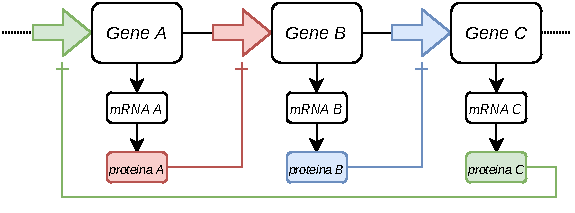
\includegraphics[scale = 1]{img/repr.pdf}
  \caption{Schema di base del Repressilator, con le frecce bidimensionali che
    rappresentano l'azione di inibizione delle proteine.}
  \label{fig:repr}
\end{figure}
Nel dettaglio del Repressilator le proteine (prodotte dai rispettivi geni che si
indicano con la prima lettera minuscola) sono, in ordine (\textit{A, B, C}):
\begin{itemize}
  \item $TetR$ prodotta dal gene $tetR$
  \item $\Lambda cI$ prodotta dal gene $\lambda cI$
  \item $LacI$ prodotta dal gene $lacI$
\end{itemize}
Il punto fondamentale, come visibile in figura \ref{fig:repr}, è capire che se
sto producendo una grande quantità di una 
certa proteina allora sicuramente non avrò produzione di quella di cui
tale proteina inibisce la trascrizione del gene e così via. Nel nostro caso se
si produce tanta \textit{proteina A} non avremo produzione di \textit{proteina
  B} e di conseguenza avremo produzione della \textit{proteina C}, ma nel
momento in cui questa terza viene prodotta cala la produzione della
\textit{proteina A} comportando la produzione della \textit{proteina B}
etc$\ldots$. Ho, in pratica, un sistema oscillatorio, con 3 proteine che si
reprimono l'una con l'altra.\\
La rappresentazione ``su carta'' di questo comportamento è abbastanza semplice,
come vedremo, modellandola tramite un insieme di equazioni differenziali. Il
problema è passare dalla teoria alla pratica. Questo sistema ``ingegnerizzato'',
di equazioni differenziali, è in grado di confermare quanto visualizzabile poi
tramite esperimenti. \\ 
Vediamo quindi come viene effettivamente costruito il sistema sperimentale
usando delle colonie di E. Coli, sfruttando la loro biologia. Nei batteri il DNA
non è, come detto, racchiuso nel nucleo ma ``circola'' in una regione, detta
\textit{nucleoide}, abbastanza accessibile all'interno del citoplasma. Nei
batteri il DNA circola in forme dette \textbf{plasmidi} quindi potenzialmente si
può sintetizzare un particolare plasmide e inserirlo in un batterio, il quale lo
userà per sintetizzare proteine. Prima è stato comunque pensato il modello
matematico e poi stato effettivamente costruito l'esperimento (al contrario
dell'ordine con cui si stanno ora spiegando quindi). \\
I due ricercatori hanno costruito due plasmidi (di cui per ora non approfondiamo
i dettagli):
\begin{itemize}
  \item un plasmide che codifica il\textit{ Repressilator}, ovvero che contiene
  i 3 geni che codificano le 3 proteine. Prima di ogni gene si ha attaccata una
  \textit{zona di induzione} 
  \item un plasmide che codifica un \textit{Reporter}, che codifica una
  particolare proteina, detta \textbf{green fluorescent protein
    (\textit{Gfp})}. La \textit{Gfp} è una proteina usata spesso in quanto fa si
  che un certo sistema diventi fluorescente, di colore verde, una volta che
  viene illuminato con una certa luce (un laser ad una determinata
  frequenza). Questo plasmide fa si che, quando $TetR$ è presente in abbondanza
  la trascrizione del gene \textit{gfp} viene bloccata e quindi diminuisce la
  quantità di \textit{Gfp}. Quindi, come $TetR$ oscilla per il sistema di
  \textit{mutua repressione}, si vedrà al microscopio un'oscillazione della
  fluorescenza della colonia di batteri. 
\end{itemize}
Ricordiamo che la fluorescenza è in realtà abbastanza comune in natura.\\
Si ha un ulteriore ``trucco''. Se si lascia una colonia di E. Coli senza alcun
controllo si avrebbe che ogni batterio inizierebbe il ciclo per conto suo, in
modo non sincrono, impedendo una corretta visualizzazione della
fluorescenza. Questo trucco è quello di inibire la produzione di $LacI$,
interferendo con la sua espressione, usando
un'ulteriore induttore, detto \textit{IPTG} ($isopropyl
\,\beta\mbox{-}D\mbox{-}1\mbox{-}thiogalactopyranoside$), e ottenendo così la
sincronia delle  
cellule dopo questo impulso iniziale di \textit{IPTG} (che poi decade
velocemente lasciando tutti gli E. Coli nello stesso stato iniziale).
\section{Il Modello Matematico}
Facciamo quindi un passo indietro e vediamo il modello matematico del
Repressilator. A partire dal modello matematico si scelgono le proteine da usare
e il comportamento da ottenere.\\
Per prevedere il comportamento complessivo del sistema ingegnerizzato, si è
quindi scritto un modello matematico che rappresenta la variazione 
dell'RNA e delle proteine espresse.\\
Per farlo indichiamo (\textbf{questo indice va sistemato}):
\begin{itemize}
  \item $\alpha_0$, numero di copie di proteine per cellula prodotte da un certo
  promotore in presenza del repressore
  \item $\alpha$, numero di copie di proteine per cellula prodotte da un certo
  promotore in assenza del repressore (sarebbe $\alpha+alpha_0$)
  \item $\beta$, rapporto tra la velocità di decadimento dell'\textit{mRNA} e
  quella della proteina 
  \item $n$, \textit{coefficiente di cooperatività di Hill} (nel caso del
  Repressilator si ha $n=2$)
  \item $m_i$, i-esimo \textit{mRNA}
  \item $p_i$, i-esima proteina che funge da repressore
\end{itemize}
L'intero sistema viene modellato con \textit{coppie di equazioni
  differenziali}. Si hanno quindi: 
\begin{itemize}
  \item un'equazione che ci rappresenta la velocità di variazione dell'i-esimo
  mRNA:
  \[\frac{\dd{m_i}}{\dd{t}}=-m_i+\frac{\alpha}{1+p_j^n}+\alpha_0\]
  Tale velocità dipende dalla quantità che già si ha di mRNA, dalla presenza
  della proteina che lo reprime (essendo sotto nella frazione al crescere il
  termine tende a zero, mentre al diminuire tende a 1)
  \item un'equazione che ci rappresenta la velocità di variazione dell'i-esima
  proteina che funge da repressore:
  \[\frac{\dd{p_i}}{\dd{t}}=\beta(m_i-p_i)\]
  Tale velocità dipende da quanto mRNA si ha a disposizione meno la quantità di
  proteina che si ha a disposizione in quel dato momento. Maggiore è la
  quantità di mRNA e maggiore è la produzione fino a che la proteina stessa
  non supera un certo livello di quantità, avendo che ``satura''
\end{itemize}
In ordine si hanno, per i geni:
\begin{table}[H]
  \centering
  \begin{tabular}{c|c|c|c}
    Indice & 1 & 2 & 3\\
    \hline
    \hline
    $i$ & $lacI$ & $ tetR$ & $\lambda cI$\\
    \hline
    $j$ & $\lambda cI$ & $lacI$ & $ tetR$ 
  \end{tabular}
\end{table}
Con ``velocità di variazione'' si intende in pratica un tasso di cambio di
concentrazione delle due \textit{specie molecolari}, ovvero un'entità che
osserviamo nel modello (in questo caso mRNA o proteina). \\
Le concentrazioni si esprimono con l'unità di misura $K_M$, ovvero il numero di
repressori necessari per dimezzare la repressione di un promotore, e il tempo in
$\tau_{mRNA}$, ovvero la velocità di trascrizione dell'mRNA, detto \textbf{mRNA
  lifetime}.
Integrando numericamente le due equazioni differenziali otteniamo un
comportamento periodico.\\
L'esperimento è stato fatto poi osservando come tutto questo diventa osservabile
in una colonia di E. Coli, opportunamente trattata, usando delle foto (dove si è
osservato anche un drift verso l'alto nel grafico oscillatorio a causa del fatto
che la colonia si espande).\\
La conoscenza di tipo matematico deve però essere trasferita in un esperimento
reale che funzioni (e i ricercatori devono essere in grado di manipolare
entrambi gli aspetti, si quello della modellazione matematica che quello più
biologico e chimico). In questo caso per ottenere oscillazioni stabili servono
determinati prerequisiti:
\begin{itemize}
  \item usare inibitori artificiali piccoli, con la cosiddetta \textit{low
    leakiness}. Promotori più corti sono più facili da manipolare e sono più
  ``veloci'' 
  \item la velocità di decadimento di proteine e mRNA doveva essere simile, per
  ottenere l'oscillazione, una meglio: una buona oscillazione. Questo si ottiene
  attaccando \textit{ssrA} ad ogni repressore 
  \item servono curve di repressione piuttosto ``ripide''. Per questo si è
  usato un promotore con multipli \textit{binding sites} (arrivando alla scelta
  di quelle date proteine), usando repressori
  cooperativi (questo è rappresentato con il parametro $n$) 
  \item usare un \textit{Reporter} non stabile, attaccando una variante di
  \textit{ssrA} a \textit{Gfp}, altrimenti si avrebbe una fluorescenza costante
\end{itemize}
\begin{figure}[H]
  \centering
  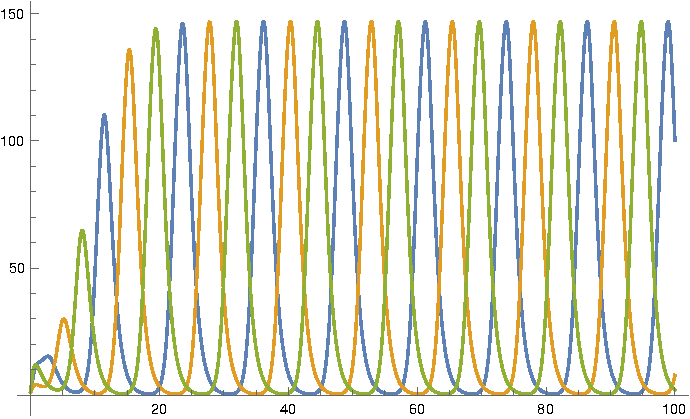
\includegraphics[scale = 0.55]{img/reprprot.pdf}
  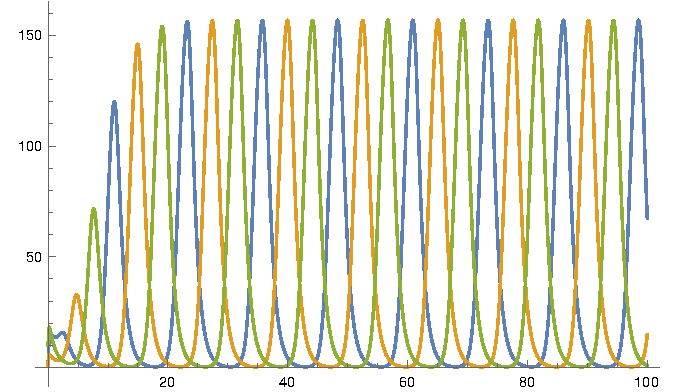
\includegraphics[scale = 0.55]{img/reprmrna.pdf}
  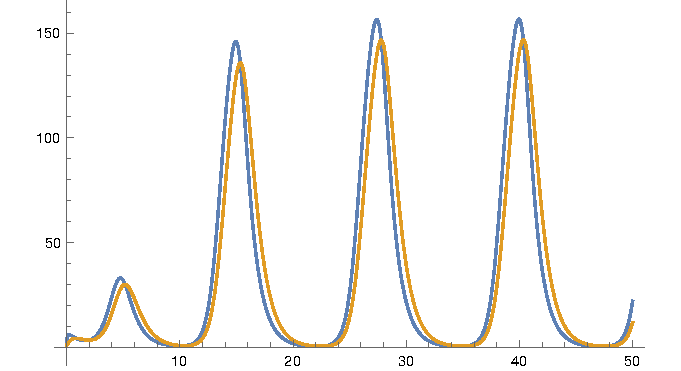
\includegraphics[scale = 0.55]{img/reprmix.pdf}
  \caption{Grafici relativi al modello del Repressilator ottenuti tramite
    Mathematica. In primis, a sinistra la quantità di 
    repressore/proteina rispetto al tempo, a destra quella di mRNA (nel primo
    caso per le 3 proteine e nel secondo per i 3 mRNA). I grafici
    cambiano drasticamente quando l'insieme dei valori dei parametri viene
    modificato. In basso le quantità di mRNA (nel caso di $tetR$) rispetto al
    repressore/proteina (in questo caso ovviamente $TetR$) associata rispetto al
    tempo. Si nota che c'è un piccolo delay nel grafico, che rappresenta il
    tempo di traduzione. Le scale dei tre grafici sono indicative. I parametri
    sono specificati nel notebook di Mathematica presente nella pagina Moodle.}   
\end{figure}
\chapter{Studio di Sistemi Biologici}
Cerchiamo ora di capire come classificare i problemi, come analizzarli e
comprenderli (anche tramite machine learning) e avere coscienza delle risorse
online disponibili per la tematica.\\
Buona parte della ricerca in biologia computazionale ha come obiettivo quello di
ottenere il passaggio dai risultati di laboratorio alle applicazioni cliniche
(ed è qualcosa di molto complesso). Per quanto ci sia interesse verso tutte le
patologie la più interessante e più studiata (soprattutto in questo corso) è il
\textbf{cancro}. Un esempio di un sistema particolare dove i tumori si
sviluppano è quello delle cosiddette \textbf{cripte coloniche (\textit{colonic
    crypts})}, avendo che questo sistema è relativamente semplice da studiare
dal punto di vista computazionale.\\
Le \textit{cripte coloniche} si trovano nell'intestino e sono delle sorta di
``pozzetti'', morfologicamente divisibili in varie aree.
Alla base delle cripte ci sono delle \textbf{cellule staminali epiteliali}, che
sono quelle che poi danno luogo ai tessuti dell'epitelio.\\
\textit{Dal punto di vista matematico tutti gli essere viventi sono di topologia
isomorfa a dei tubi.}\\
Tornando al discorso delle cellule staminali si ha che essere si suddividono e,
man mano che si suddividono tendono a spingere verso l'alto le cellule che si
trovano ``al di sopra'' di loro. Man mano che tali cellule vengono spinte
anch'esse tendono a dividersi spingendo le altre cellule verso il \textit{lumen
  della cripta}. In questo processo di suddivisione queste cellule si
differenziano e le cellule staminali danno luogo ad una progenie che possiamo,
dal punto di vista in primis computazionale, rappresentare come un
\textit{albero}. Si hanno le cellule di tipo diverso, più o meno
differenziate che continuano a salire verso la superficie dell'epitelio e poi
tendono a salire su quelli che sono detti i \textit{villi intestinali}. Questo è
un interessante processo che può essere simulato, tra i vari modi, in modo tale
che si simuli cosa accade quando le varie differenziazioni non funzionano
perché, ad esempio, si ha una cellula che ha acquisito una mutazione, mutazioni
che danno luogo ad una crescita non corretta, ad una \textit{displasia}, che è
la fase iniziale da cui poi si sviluppano i \textit{tumori del colon}. Si vuole
quindi fare queste simulazioni e farle in modo il più fedele possibile.\\
Per capire se una cellula si sta comportando in modo corretto o meno dobbiamo
misurarne il comportamento. In primis vogliamo misurare due cose, tra le tante:
\begin{enumerate}
  \item \textbf{gene expression}
  \item \textbf{gene alterations}, ovvero le varie mutazioni del genome, le
  cosiddette le \textit{copy number variations} etc$\ldots$
\end{enumerate}
La tecnologia a disposizione per queste tematiche si è molto evoluta ma tra le
tante tecnologie si segnalano:
\begin{itemize}
  \item \textit{microarrays} per l'espressione genica, usati però molti anni fa
  essendo una delle prime tecnologie per misurare, in modo indiretto ma
  parallelo, l'espressione dei geni
  \item \textit{Next Generation Sequencing (NGS)} per praticamente qualsiasi
  cosa, anche per l'espressione genica, in modo diretto tramite particolari
  esperimenti (\textbf{nella rec non ho capito il nome di tali
    esperimenti}). NGS ha avuto molta fama da circa il 2006 in poi, con il
  monopolio poi di Illumina, anche se di recente si hanno nuove tecnologie che
  stanno rivoluzionando il settore (che producono read più lunghe)
\end{itemize}
\section{Microarrays}
Parliamo un secondo dei \textbf{microarrays}.\\
Questa è una tecnologia non più utilizzata, essendo di inizio anni duemila, che
però è utile per spiegare come si procede a fare un certo tipo di misure, con
una tecnologia che è stata poi ripresa da Illumina.\\
Questo strumento si basa su una griglia a cui sono attaccate delle ``sonde''
lunghe circa 25 nucleotidi e venivano usati per caratterizzare i geni. Si
producono infatti segnali luminosi di diversa intensità e diversa lunghezza
d'onda in una griglia, da cui si può ricavare una griglia numerica che dà
informazioni in merito alla luce di ogni punto.\\
I Microarrays sono prodotti da Affymetrix e hanno circa $10^5$ sonde, che
caratterizzano tutti i geni che interessano. \\
Si ottiene quindi un'immagine contiene una griglia, dove in ogni punto si
produce un segnale luminoso di diversa intensità e lunghezza d'onda dalla quale
si ricava, misurando i segnali luminosi, una \textbf{matrice di espressione},
dove:
\begin{itemize}
  \item le righe sono i geni/trascritti
  \item le colonne sono misure numeriche
\end{itemize}
e si ha, per ogni sonda, quanto e come è luminoso il tal punto nella griglia.\\
Si prende quindi del DNA, lo si ``denaturalizza'', ovvero lo si sgroviglia, e lo
si versa direttamente sulla griglia. Il DNA (ma potrebbe essere anche essere
RNA) viene versato sulla griglia e si ``attacca'', grazie alle sue proprietà
chimiche, alle sonde (in pratica le parti di DNA/RNA si attaccano alle sonde a
loro complementari). Il trucco è quello di ``colorare'' i pezzi di DNA e RNA e
questo si fa usando, come nel caso del Repressilator, delle proteine
fluorescenti, verdi e rosse, usando quindi processi biochimici per attaccare ai
pezzi di DNA/RNA queste proteine, che emetteranno fluorescenza una volta colpite
da un laser. Si può quindi vedere, in ogni punto della griglia, se si ha un
segnale rosso o uno verde, misurandone l'intensità, ottenendo una misura di
quanto materiale genico si sia attaccato in ogni punto della griglia.\\
Vediamo quindi come si utilizza questo tipo di tecnologia per fare delle misure
di \textit{geni differenzialmente espressi in diverse condizioni}.\\
Si hanno delle cellule in una certa condizione e altre in un'altra condizione
(magari, per esempio, una delle due condizione è una crescita in ambiente con
pochi nutrienti o in un ambiente con temperature estreme, sia alte che basse con
associati shock termici per le cellule). La prima condizione è normalmente uan
\textit{condizione standard}, detta \textit{condizione wild-type}, mentre la
seconda è la condizione che si vuole studiare.\\
Si hanno due fasi per l'esperimento:
\begin{enumerate}
  \item si estrae dalle cellule nelle due condizioni l'RNA, che descrive ciò che
  le cellule stanno in quel momento esprimendo, quali proteine stanno
  sintetizzando, etc$\ldots$ Dall'RNA, che nel dettaglio è \textit{mRNA},
  estraggo il \textit{cDNA}, al quale poi attacco le proteine per la
  fluorescenza. Si procede quindi con la cosiddetta \textit{ibridazione}, ovvero
  si prende il materiale genetico con fluorescenza e si immerge il
  microarrays in questa soluzione, procedendo poi alla scansione con il
  laser
  \item nella griglia si ottiene quindi che del materiale genico delle cellule
  nella prima condizione si attaccano ad alcune sonde mentre quella delle
  seconda condizione ad altre. In ogni punto della griglia o non si attacca
  niente (non avendo che le cellule esprimono quanto necessario per quel punto)
  o si attacca solo l'RNA di una delle due condizioni o si attaccano entrambi.
  Usando poi i laser per le due fluorescenze si ottiene l'immagine, avendo punti
  senza luce (nero), alcuni con luce verde, alcuni con luce rossa, a seconda
  della prevalenza del materiale che viene da una delle due condizioni (se
  simili si ha una luce tendente al giallo). Una volta prodotta l'immagine si
  produce l'output numerico delle intensità. 
\end{enumerate}
L'esperimento può essere ripetuto più volte, ottenendo una serie di matrici
numeriche che possono unite in vari modi, ottenendo la \textbf{gene expression
  data matrix} finale, coi vari \textbf{gene expression levels}, i livelli di
espressione di ogni gene, ricordando che ogni gene è codificato da più
sonde. Per ogni gene ho la \textbf{differenza di espressione} tra le due
condizioni.
\begin{definizione}
  Si definiscono due geni come \textbf{differenzialmente espressi} se sono due
  geni che ho risultano rossi o verdi (???).
\end{definizione}
Se tale matrice finale è ottenuta variando solo i tempi e mantenendo 
fisse le altre condizioni sperimentali si ha che essa rappresenta il
\textit{time-course of genes expression}.\\
Sui risultati si può fare \textbf{data mining}, usando tecniche di machine
learning. \\
Si vuole fare clustering di geni o sonde che esibiscono un comportamento simile
dato un insieme di condizioni sperimentali o ambientali. Per farlo si hanno vari
tool (molti dati disponibili sulla repository NCBI, soprattutto nella
sotto-repository GEO) ma molti studi richiedono
una sistemazione finale non banale in merito a ``rumori'' e variazioni di
protocollo nei laboratori. \\
Ad esempio, in un esperimento di espressione genica si hanno vari step:
\begin{enumerate}
  \item dopo la ``pulizia'' della matrice (tramite controllo qualità) si usano
  alcune analisi standard, ragionando magari su vari \textit{time points}
  discreti: 
  \begin{itemize}
    \item \textit{clustering}, tramite K-Means, per ogni punto, ottenendo dei
    vettori che rappresentano il comportamento  di un gene in un certo tempo. Si
    ottengono cluster di traiettorie. Si raggruppano geni con simile profilo di
    espressione 
    \item \textit{enrichment}, che altro non è l'operazione in cui si prendono i
    dati e gli si associano informazioni, tramite \textit{Gene Ontology (GO)
      Terms}. La GO è un elenco di nomi con ID unico e oggi come oggi i geni
    noti sono stati già etichettati coi termini dalla GO. Vengono annotati i
    termini sovrarappresentati in un cluster. L'etichettatura fa si che quando
    ho gruppi di geni posso usare tecniche statistiche, come il \textbf{test
      esatto di Fisher}, per estrarre i termini più rappresentativi, quelli più
    presenti e descrittivi di un gruppo. In 
    questo modo, un cluster può essere associato ad alcuni termini
    ``rappresentativi'', che possono indicare una certa caratterizzazione
    funzionale e ipotesi di associazioni tra geni e un certo comportamento (se
    questo non fosse già annotato). Questa tecnica è detta \textbf{associazione
      a delinquere}, in quanto si ``accusano'' geni di essere associati ad
    altri, comportandosi in modo simile
  \end{itemize}
\end{enumerate}
\textbf{Su slide, parte 2 a pagina 13, grafici di un esperimento e annessi
  termini da GO}.\\  
Vediamo nel dettaglio GO\footnote{\url{www.geneontology.org}}
che è appunto un \textit{vocabolario
  controllato/ontologia} che è diventato la chiave per condividere le conoscenze
biomolecolari, in particolare per i geni e i prodotti genici. È nata negli anni
novanta a Berkeley mettendo insieme una serie eterogenea di conoscenze
proveniente da vari ambienti. È nata cercando una nomenclatura standard per la
genetica della Drosophila. È stata ottenuta con lo sforzo di informatici,
biologi, filosofi etc$\ldots$ usando, in primis, l'IA simbolica (usata per le
ontologie, ovvero modi di descrivere in modo simbolico una serie di concetti).\\
Ogni temrine in GO ha un codice numerico univoco.\\
Si hanno tre sotto-ontologie, ognuna con una struttura gerarchica a DAG
(\textbf{su slide immagine di struttura}):
\begin{enumerate}
  \item \textbf{MF} (\textit{Molecular Function}), per le attività biochimiche
  il tipo molecolare
  \item \textbf{BP} (\textit{Biological Process})
  \item \textbf{CC} (\textit{Cellular Component})
\end{enumerate}
Lato tecnico si ha, sotto GO, un linguaggio logico (stile \textit{Prolog}), con
un insieme di relazioni, termini e costanti di un linguaggio.\\
GO non è l'unica ontologia a disposizione, anzi se ne hanno centinaia ma meno
importanti. GO offre delle API e si hanno tool come \textit{AmiGO} per
recuperare informazioni.
\section{Next Generation Sequencing}
Dopo aver parlato di \textit{microarrays} parliamo di \textbf{Next Generation
  Sequencing (\textit{NGS})}.\\
Vediamo quindi le nuove tecnologie di sequenziamento. Diciamo ``nuove'' perché
le prime tecnologie di sequenziamento sono datate anni cinquanta con il metodo
Sanger per sequenziare proteine. Più avanti, nei primi anni settanta, si sono
sviluppati i primi progetti per sequenziare DNA e RNA, studiando i virus (in
quanto molto piccoli). Nel 1995 poi si è riuscito a sequenziare interamente un
batterio, l'H. Influenza.\\
Nel 1990 si svilupparono vari metodi per il sequenziamento high-throughput,
progetti che permisero di lanciare lo \textit{Human Genome Project}, che fu
completato nel 2000 quando pubblicarono in estate la prima bozza di genoma
umano. \\
Le prime macchine semiautomatiche per il sequenziamento furono le
\textit{Biosystems ABI 370} ma oggi si usano i macchinari \textit{Illumina}. Un
macchinario \textit{Illumina HiSeq 2000} corrisponde, in termini di prestazioni,
a 23648 \textit{Biosystems ABI 3730}, degli anni novanta.\\
Si hanno due tipi di attività parlando di NGS:
\begin{enumerate}
  \item \textbf{Wet-Lab Activity}, ovvero le attività di raccolta dati/misure
  del materiale biologico, ovvero del vero e proprio sequenziamento tramite
  tecniche biochimiche. Si ha
  quindi la frammentazione e l'estrazione dei frammenti di DNA e RNA, il
  sequenziamento dei frammenti e la generazione delle read (con le 4 basi e
  caratteri extra per le ambiguità o i dati mancanti)
  \item \textbf{Dry-Lab Activity}, ovvero le attività di assemblaggio. Si ha il
  salvataggio delle read, che sono tantissime (con conseguenti problemi di
  storage), e l'assemblaggio delle 
  read (che sono \textit{short read}) in \textit{contings}, che sono read più
  lunghe. Dai contings si passa poi alla sequenza più ampia che stiamo
  sequenziando (anche un intero cromosoma o un intero genoma). Quest'ultimo è un
  problema prettamente algoritmico
\end{enumerate}
Attualmente le tecnologie NGS producono read di lunghezza limitata (Illumina
produce read da 70/150 basi circa) e il costo è
proporzionale al numero delle read prodotte. Il parametro più importante è il
parametro di \textbf{coverage}, ovvero il \textit{depth of sequencing}, ovvero
quante sequenze si hanno che coprono la medesima zona di DNA. Avere un alto
coverage riduce il rischio di errore di sequenziamento ma un alto coverage
implica alti costi e quindi è un parametro che va ``bilanciato''. Sono limiti
tecnologici.\\ 
Il costo di sequenziamento, dal 2006, è sceso di molto e siamo ora intorno ai
1000 dollari per genoma (mentre nel 2000 eravamo intorno ai 100000 dollari). Nel
2006/2007 sono state infatti introdotte le tecnologie Illumina, molto più
economiche. Anche nel 2015 si ha avuto un abbassamento e ora siamo in un
plateau sui 1000 dollari. Inoltre, rispetto alla \textbf{legge di Moore}, il
costo per genoma è sceso molto rispetto alla legge stessa.\\
Si hanno anche nuovi macchinari di sequenziamento, con una diversa tecnologia di
base rispetto ad Illumina:
\begin{itemize}
  \item \textbf{Single Molecule Real Time (\textit{SMRT}) sequencing}, che
  sequenzia una molecola di DNA o RNA per volta
  \item \textbf{Nano Sensing sequencing}, che permette di avere un sequenziatore
  piccolissimo collegabile via USB al proprio computer. Si hanno problemi
  relative al software che ricostruisce le sequenze, avendo percentuali di
  errore veramente molto (con errori di natura diversa da quelli di Illumina,
  che sono comunque percentualmente molto minori)
\end{itemize}
Tra i tipi di sequenziamento abbiamo:
\begin{itemize}
  \item \textbf{Whole-Genome Sequencing}, per interi genomi, anche
  \textit{de-novo} (ovvero senza un \textit{reference} preesistente)
  \item \textbf{Exome Sequencing}, per solo le parti di genoma codificanti
  (infatti solo alcune parti, poche, del genoma codificano le proteine mentre il
  resto del genoma non si sa bene a cosa serva)
  \item \textbf{Target (re)sequencing}, per zone specifiche del genoma, spesso
  sono misure secondarie dopo un Whole-Genome Sequencing per zone ``dubbie'' o
  che servono in quantità maggiore (magari perché legate a certe proteine)
  \item \textbf{RNA-seq}, sequenziando RNA, usando le tecnologie NGS per
  determinare l'attività dell'espressione genica (studiando che proteine sta
  generando una cellula etc$\ldots$), caratterizzando i trascrittomi. Si evitano
  i vari passaggi che si facevano con i microarrays, che davano una misura
  indiretta per di più (l'intensità della luce etc$\ldots$). Qui basta
  sequenziare e poi contare le read di un particolare RNA
  \item si hanno ora molte altre \textbf{*-seq} in letteratura. Ad esempio
  \textbf{ATAC-seq (\textit{Assay for Transposase-Accessible Chromatin using
      sequencing})}, che è legato allo studio della conformazione
  tridimensionale del DNA, delle \textit{aperture/chiusure della cromatina},
  studiando cosa è trascrivibile in un dato istante oppure no
\end{itemize}
\subsection{Dal Sequenziamento alle Analisi}
Dopo il sequenziamento vogliamo vedere come tutte queste informazioni possono
essere usate per fare analisi su come si comportano alcuni processi biologici,
in particolare il \textbf{comportamento dei tumori}.\\
Una delle cose che si possono fare è prendere campioni di tumori da più pazienti
e ricostruire le parti comuni dei tumori stessi, per ottenere i vari sottotipi
del tumore. Questo studio è legato a certi
tipi di tumore (si hanno circa 40 tipi di tumore in totale con i relativi
sottotipi).  \\
Un'altra cosa che si può fare è analizzare il tumore di un individuo che si è
poi suddiviso in \textit{primario} e \textit{metastatico}, costruendo una
\textbf{filogenia tumorale}. Per farlo si prendono campioni del tumore e si fa
una cosiddetta \textbf{bulk analysis}, ovvero un'analisi aggregata prendendo un
tessuto ed estraendo il DNA dal tessuto, ottenendo materiale genico da diverse
cellule (perdendo l'individualità di ogni cellula ottenendo una misura
``media''). Si hanno poi vari algoritmi per ottenere la filogenia, più o meno
complessi, ricostruendo \textbf{l'albero della filogenia tumorale}, che parte da
un tumore iniziale e poi presenta le varie differenziazioni che si sono
sviluppate di quel tumore.
\section{Single-Cell Analysis}
In merito all'ultimo aspetto della sezione precedente, più di recente, si sono
sviluppate tecnologie più sofisticate dal punto di vista chimico e fisico, per
isolare singole celle prese da un campione. In questo modo si ha una
rappresentazione più precisa di come sono fatte le popolazioni di cellule in un
campione. Si usano poi algoritmi di filogenia per ricostruire le
\textit{evoluzioni clonali}. Questa tecniche sono dette
appunto\textbf{tecniche di Single-Cell Analysis}. Si parte quindi sempre da un
sequenziamento ma associato a singole cellule.\\
La Single-Cell Analysis è cruciale in questo periodo e può essere usata per
tantissimi progetti. In Bicocca si hanno progetti di \textbf{Metagenomica}, dove
si isolano organismi da popolazione di organismi, sequenziando il singolo
organismo (ma sequenziandone tanti). Viene fatto per studiare le popolazioni
microbiche nelle falde acquifere o negli acquedotti. Si isolano organismi noti
da organismi non noti, per riuscire poi a distinguerli e catalogarli,
etichettandoli con il rispettivo materiale genico (il \textit{corredo
  genomico}). Questo non era possibile con questa facilità prima dell'uso della
Single-Cell Analysis. \\
Attualmente è comunque una tecnica molto costosa (contando che in un esperimento
si sequenziano migliaia di singole cellule).
\section{Risorse Online}
Vediamo quindi una breve carrellata di risorse online importanti:
\begin{itemize}
  \item \textbf{NCBI (\textit{National Center for Biotechnology Informationy})},
  dove si hanno tutte le varie risorse più usate, ad esempio \textit{PubMed}
  (per la ricerca di paper), \textit{Blast} (uno dei più famosi allineatori di
  sequenze, nonché uno dei software informatici più usati al mondo),
  \textit{Gene} (un importante database) etc$\ldots$ Si hanno inoltre modalità
  per trasmettere i risultati di ricerche, scaricare dati, informazioni su
  come interfacciarsi senza usare l'interfaccia web (per fare programmaticamente
  analisi più ampie tramite API), varie risorse per imparare le tecnologie,
  tutorial etc$\ldots$ 
  \item \textbf{BioModels}, dove si trovano modelli di sistemi biologici di
  varia natura (come vari modelli per il Repressilator). Tali modelli sono
  disponibili in vari formati (ad esempio per MATLAB etc$\ldots$) e sono
  simulabili  
  \item \textbf{BioCyc}, un database storico che contiene una rappresentazione
  di tutte le reazioni metaboliche di un organismo. Era nato originariamente per
  il metabolismo di E. Coli ed è stato poi generalizzato a vari organismi
  \item \textbf{KEGG (\textit{Kyoto Encyclopedia of Genes and Genomes})}, un
  portale giapponese che fornisce un insieme di database relativi a vari dati di
  carattere biologico. Fornisce delle API, di recente riscritte per usare la
  terminologia REST, e altri tool
  \item \textbf{Pathway Commons}, un database per pathway metaboliche o
  regolatorie pubbliche
  \item \textbf{Firehose e Firebrowse}, un'interfaccia semplificata ad un
  database complesso chiamato \textbf{TCGA (\textit{The Cancer Genome
      Atlas})}. TCGA è un database, ora parte di NCBI, che raccoglie i dati di
  esperimenti che hanno misurato variazioni nel genoma relativi a tumori, e
  permette di scaricare in modo semplificato i vari dati relativi a tali tumori
\end{itemize}
Ovviamente questa lista è solo introduttiva.
\end{document}

% LocalWords:  clock  differenzialmente sequenziatore reference trascrivibile
% LocalWords:  REST
